\documentclass[xcolor=table]{beamer}
\usepackage[orientation=portrait,size=a0,scale=1.225]{beamerposter}
\usepackage{polyglossia}
\setdefaultlanguage{english}
\usepackage{fontspec}
\usepackage{graphicx}
\usepackage{multicol}
\usepackage{fancyhdr}
\usepackage{tikz}
\usepackage{ulem}
\usepackage{ragged2e}
\usepackage[table]{xcolor}
\usepackage{rotating}
\usepackage{xstring} % for string operations

%\setbeamertemplate{caption}[numbered] 

\let\olditem\item
\renewcommand\item{\olditem\justifying}

%%%%%%%%%%%%%%%%%%%%
% Document started %
%%%%%%%%%%%%%%%%%%%%

%\mode<presentation>{%
\usetheme{Pasky-poster}
%\usecolortheme{ComingClean}
\usecolortheme{Entrepreneur}
%\usefonttheme{serif}
%}
\setlength{\columnsep}{4em}

\title{YodaQA: A Modular Question Answering System Pipeline}
\author[baudipet@fel.cvut.cz]{Petr Baudiš}
\institute{Department of Cybernetics, Czech Technical University, Prague}
\postermarker{ICS20}
%\date{May 15th, 2014}

\begin{document}
\begin{frame}[fragile]{}

  \begin{columns}[t]
    \column{.95\textwidth}
  \begin{multicols}{2}
    \large
    \justifying
    \setlength{\fboxsep}{15pt}%
%
    \colorbox{yellow!20!white}{\parbox{.96\columnwidth}{%
    \alert{\bfseries\sffamily Goal:} Answer naturally phrased factoid questions,
    using both structured (e.g. Freebase) and unstructured (e.g. Wikipedia)
    knowledge bases.
    }}

    \columnbreak

    \colorbox{green!15!white}{\parbox{.96\columnwidth}{%
    \alert{\bfseries\sffamily Contribution:} A universal framework that
    allows integration of diverse state-of-art approaches within a common pipeline.
    }}
  \end{multicols}
  \vspace{2ex}
  \end{columns}

  \begin{columns}[t]
    \column{.45\columnwidth}

    \begin{block}{Background}

      \begin{columns}[t]
	\column{.45\columnwidth}
	\begin{block}{Question Answering}
	\setlength{\parskip}{0.5ex}

		Unstructured user query $\to$ narrow text snippet answering the query.

		\structure{\dots\ vs.\ linked data graph search:} requires a precisely structured user query.

		\structure{\dots\ vs.\ a search engine:} returns a whole document or passage.

The Question Answering task is already part of the \alert{Google Search}
interface
or personal assistants like \alert{Apple Siri}, and with the high
profile \alert{IBM Watson} Jeopardy! matches
it has became a benchmark of progress in AI research.

As we are interested in a general purpose QA system, we will consider
an \alert{``open domain'' factoid} question answering, rather than
domain-specific applications (though we have domain flexibility as
one of our goals).
	\end{block}

	\column{.45\columnwidth}
	\begin{block}{Previous Work}
	\setlength{\parskip}{0.9ex}

The most popular approach in QA research has been restricting
the task to querying \alert{structured knowledge bases}, typically using the
RDF paradigm and accessible via SPARQL\@.  The problem can
be then rephrased as \alert{machine translation} from free-text user query
to a structured query (SPARQL, $\lambda$-expr).

When relying on unstructured knowledge bases, a common strategy is to offload
the information retrieval on an external high-quality \alert{web search} engine
like Google or Bing; we avoid this for the sake of domain flexibility and
reproducibility of results.

\structure{Notable open source systems:} OpenEphyra, OAQA, WatsonSim, Jacan\-a, OpenQA.
	\end{block}
      \end{columns}
    \end{block}

    \vspace{1ex}
\resizebox{\columnwidth}{!}{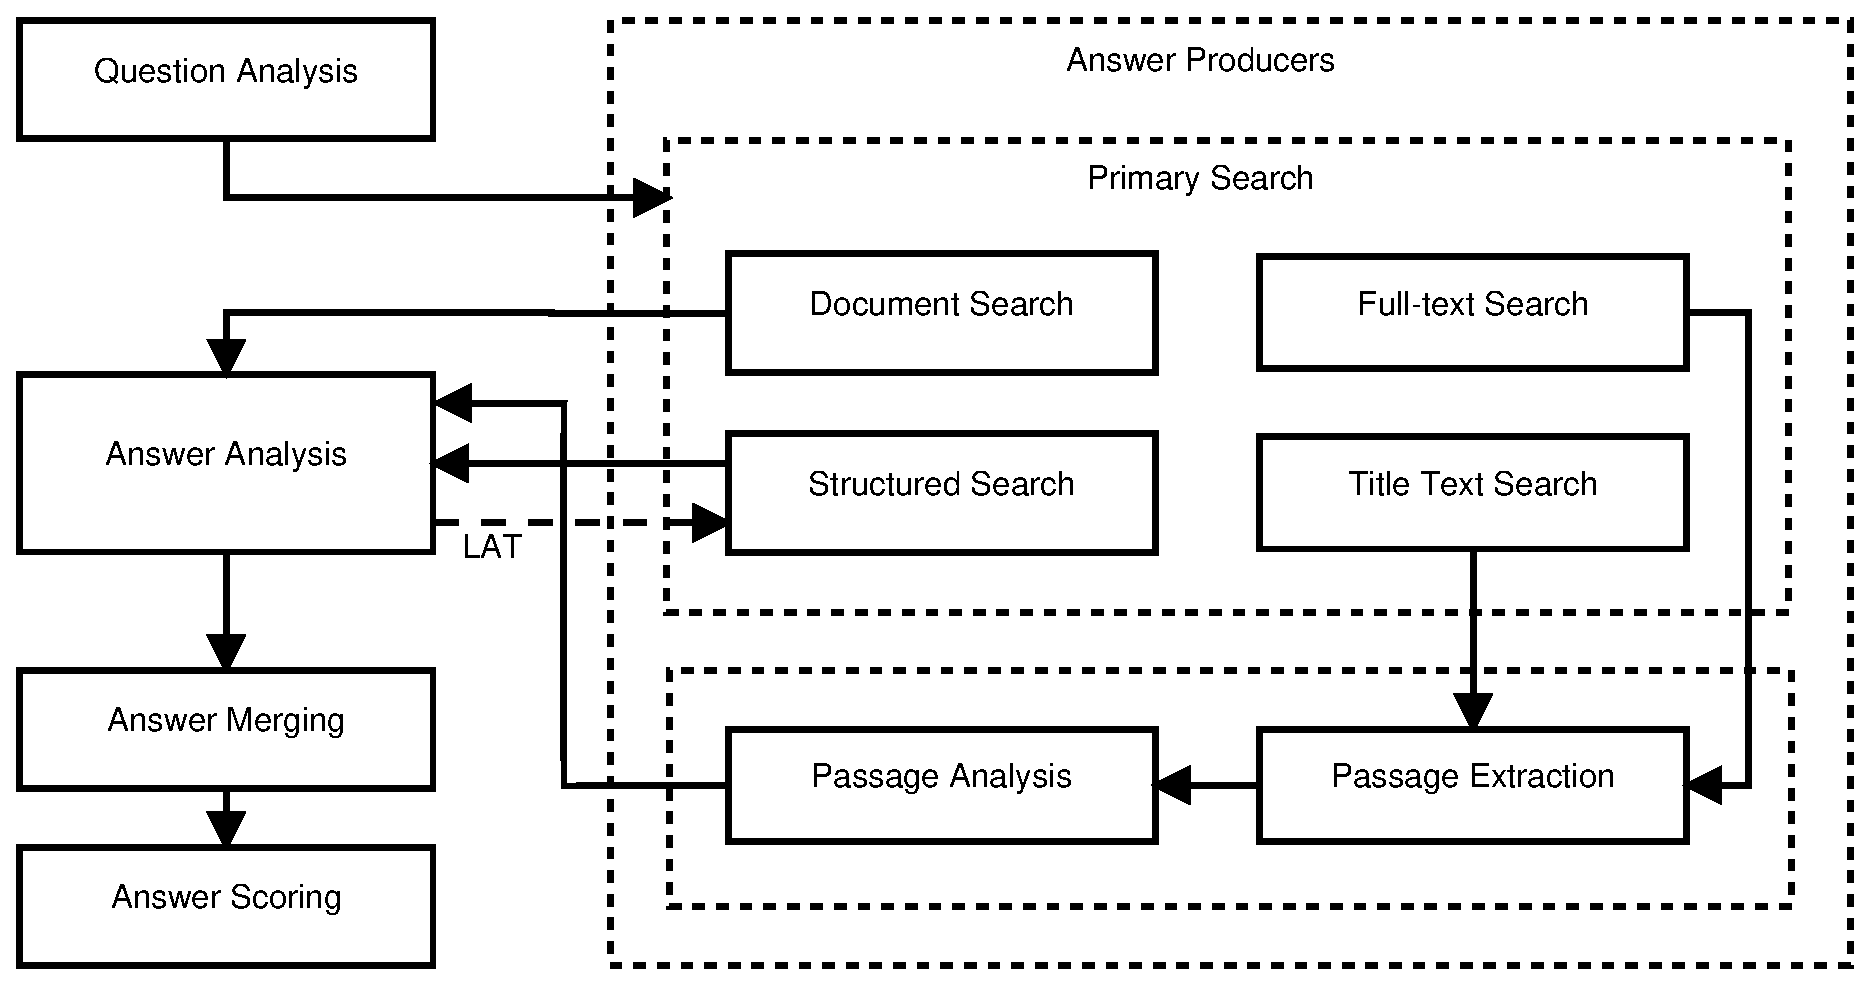
\includegraphics{../yodaqa-arch.eps}}
    \vspace{-0.5ex}

\begin{columns}[t]
\column{.45\columnwidth}

\centering
\footnotesize
\begin{tabular}{|p{3.6cm}p{13cm}|}
\hline
Text & \hspace{0pt}\alert{Who wrote Ender's Game?} \\
Q. Analysis & \textbf{Focus:} who; \textbf{SV:} wrote; \textbf{LAT:} person \\
Clues & Ender's Game \textbf{(concept clue)}, wrote \\ \hline

DBpOnt. & \textbf{author:} Orson Scott Card, \textbf{pub.:} Tor Books\\
%DBpProp. & \textbf{cover artist:} John Harris, \textbf{Caption:} 2005, \dots \\
Freebase & \textbf{Author} Orson Scott Card, \textbf{Characters} Valentine Wiggin, Hive Queen, \dots \\
%Concepts & \textit{enwiki} Ender's Game \\
Fulltext %
	%& \textbf{Query:} \texttt{+("wrote" OR titleText: "wrote")\^{}1.0 +("ender's Game" OR titleText:"ender's Game")\^{}1.1  ("wrote ender's Game "\textasciitilde4)\^{}2.1} \dots \\
	& Ender's Game (series), Ender's Game, Ender's Game (film), Jane (Ender's Game), List of Ender's Game series planets \\
	& \textbf{Sample picked passages:} {\footnotesize Elaborating on characters and plot lines depicted in the novel, Card later wrote additional books to form the Ender's Game series.} \\
	%& \dots {\footnotesize Valentine wrote an essay here comparing the priestly class to the skeletons of small vertebrates before Speaker for The Dead.} \\
Titles & Ender's Game, List of Ender's Game characters, Jane (Ender's Game), Ender's Game (short story), Ender's Game (film) \\
	& \textbf{Sample first passage:} {\footnotesize "Ender's Game" is a 1985 military science fiction novel by American author Orson Scott Card.} \\
Doc. & Ender's Game (series), Orson Scott Card, Worthing Inn, Jane (Ender's Game), \dots \\ \hline

\hspace{0pt}\alert{Orson Scott Card} & Structured search LAT \textit{author} (Wordnet hn. \textit{communicator}, \textit{person}, \textit{maker}, \textit{creator}); DBpedia LAT \textit{writer}; NER LAT \textit{person} \\
	& Successful type coercion match\textbf{!}, ``sharp'' (exact specific) match from NER LAT\textbf{!} \\
	& \textbf{occurences:} 19\textbf{!}, \textbf{origins:} document title, concept\textbf{!}, first passage, noun phrase, named entity, multiple origins, \textbf{other:} adjecent to a concept clue mention, no clue text overlap\textbf{!} \\
\hspace{0pt}\alert{Jane} & Structured search LAT \textit{character} (Wordnet hn. \textit{imaginary being}, \textit{creativity}, \textit{person}, \textit{message} and 36 others); NER LAT \textit{person} \\
	& Successful type coercion match\textbf{!}, ``sharp'' (exact specific) match from NER LAT\textbf{!} \\
	& \textbf{occurences:} 4, \textbf{origins} document title, first passage, noun phrase, named entity, multiple origins,
	\textbf{other:} no clue text overlap\textbf{!} \\ \hline

Final Answers & \hspace{0pt}\alert{Orson Scott Card} (0.99), Neal Shusterman (0.96), American author O. S. Card (0.96), List of Ender's Game series planets (0.94), Gavin Hood (0.94), Jane (0.91), \dots \\ \hline
\end{tabular}

\column{.45\columnwidth}

\centering
\footnotesize
\begin{tabular}{|p{3.6cm}p{13cm}|}
\hline
Text & \hspace{0pt}\alert{What is the name of the famous dogsledding race held each year in Alaska?} \\
Q. Analysis & \textbf{Focus:} name; \textbf{SV:} held; \textbf{LAT:} race
	(by Wordnet hypernym: \textit{contest}, \textit{event}, \textit{biological group}, \textit{canal} and 9 others) \\
Clues & name, Alaska \textbf{(concept clues)}, race, held, famous, dogsledding, race, year \\ \hline

DBpOnt. & \textbf{area:} 1717854.0, \textbf{country:} United States \\
DBpProp. & \textbf{West:} Chukotka, \textbf{Income Rank:} 4, \dots \\
%Freebase & \textbf{Date Founded} 1959-01-03, \textbf{Capital} Juneau, \dots \\
Concepts & \textit{enwiki} Alaska, Name \\
	& \textbf{Sample picked passages:} Various races are held around the state, but the best known is the Iditarod Trail Sled Dog Race, a 1150 mi trail from Anchorage to Nome (although the distance varies from year to year, the official distance is set at 1049 mi). \\
	%& \dots Automobiles typically have a binomial name, a "make" (manufacturer) and a "model", in addition to a model year, such as a 2007 Chevrolet Corvette.\\
Fulltext %& \textbf{Query:} \texttt{("the name of the famous dogsledding race held each year in Alaska" OR titleText:\dots)\^{}2.7 +("name" OR titleText:"name")\^{}2.6} \dots \\
	& List of New Hampshire historical markers \\
Titles & Name of the Year, Danish Sports N. of the Y., List of organisms named after famous people, Alaska!, Alaska, Race of a Thousand Years \\
	%& \textbf{Sample first passage:} The 2000 Race of a Thousand Years was an endurance race and the final round of the 2000 American Le Mans Series season. \\
Doc. & List of New Hampshire historical markers \\ \hline

\hspace{0pt}\alert{2000 Race of T. Y.} %
	& DBpedia LAT \textit{automobile race}, \textit{auto race in australia}, \textit{new year celebration}, \textit{quantity} LAT \\
	& Successful type coercion match\textbf{!}, ``sharp'' (exact specific) match\textbf{!} \\
	& \textbf{occurences:} 1, \textbf{origins:}  first passage, noun phrase, \textbf{other:} adjecent to an LAT clue mention\textbf{!}, containing clue text \\
\hspace{0pt}\alert{Iditarod Trail Race} %
	& DBp. LAT \textit{sport}, \textit{sport in alaska}, \textit{alaska}, \textit{winter sport}, \textit{attraction}; (not \textit{race}) \\
	& Successful tycor.\ match, loose match by generalization of \textit{attraction} to \textit{social event}\textbf{!} \\
	& \textbf{occurences:} 1, \textbf{origins}   passage by various clues, noun phrase,
	\textbf{other:} suff.\ by clue text \\ \hline

Final Answers & The 2000 Race of a Thousand Years (0.97), --01-03 (0.94), List of New Hampshire historical markers (0.93), a binomial name, a "make" (manufacturer) and a "model", in addition to a model year, such as a 2007 Chevrolet Corvette (0.90), \alert{the Iditarod Trail Sled Dog Race} (0.89), Various races (0.83), \dots \\ \hline
\end{tabular}
\end{columns}

    \column{.45\columnwidth}

    {\structure{Keywords:}
	Question answering, information retrieval, information extraction,
	linked data, natural language processing, Apache UIMA,
	software engineering.}
    \vspace{3ex}

    {%
	    \centering
	    \large {\bfseries
	    \alert{Ask for a live demo!}
	    } (\structure{\large{}live.ailao.eu})
	    \par
    }

    \vspace{3ex}

    \begin{block}{The YodaQA Framework}
      \begin{multicols}{2}
	%\setlength{\parindent}{1.2em}
	\setlength{\parskip}{1ex}
	\vspace{-1ex}

	\alert{\bfseries\sffamily Paradigm:} We are interested in \alert{combining
	different approaches}, using different
	question representations, answer sources and scoring features.
	Our baseline is \alert{domain flexible}
	and we strongly prefer machine learning to hand-crafted heuristics.

	%\columnbreak

	\alert{\bfseries\sffamily Platform:} Mainly Java, using the Apache UIMA
	framework and DKpro family of adapters to various NLP tools.

	\alert{\bfseries\sffamily Availability:}
	Publicly available free software under the
	Apache licence at \structure{\url{https://github.com/brmson/yodaqa}}.
      \end{multicols}

    \end{block}

    \begin{block}{The Baseline QA Pipeline}

    \justifying
The basic pipeline flow is much inspired by the Deep\-QA model
of IBM Watson.  Throughout the flow, answer features
are gradually accumulated.
%and some results of early flow stages (especially
%the question analysis) are carried through the rest of the flow.

      \begin{columns}[t]
	\column{.45\columnwidth}

\begin{block}{Question Analysis}
	\begin{itemize}
		\item \textbf{Focus}
			\begin{itemize}
				\item What was the first \alert{book} written by Terry Pratchett?
				\item The \alert{actor} starring in Moon?
			\end{itemize}
		\item \textbf{LAT} (Lexical Answer Type)
			\begin{itemize}
				\item \alert{\sout{Where}} is Mount Olympus? \alert{location}
			\end{itemize}
		\item \textbf{Clues} (search keywords/phrases)
			\begin{itemize}
				\item POS and constituent token whitelist
				\item Named entities
				\item Focus and the NSUBJ constituent
				\item \textbf{Concepts:} \texttt{enwiki} article titles
			\end{itemize}
	\end{itemize}

	%\vspace{3ex}

	\centering
\colorbox{green!30!white}{\textbf{Outcome:} Question representation}% in QuestionCAS}
\end{block}

	\column{.45\columnwidth}

\begin{block}{Answer Production}
%	\centering
%		Several answer production pipelines \\ run independently in parallel.
		%(custom flow controller developed).

%	\vspace{2ex}

	\begin{itemize}
		\item Passage-yielding enwiki search
			\begin{itemize}
				\item \textit{Fulltext:} Full-text and title search, \\ \alert{passages containing clues} are considered
				\item \textit{Title-in-clue:} Title search for clues, \\ \alert{initial passage} is considered
				\item Passages are parsed, \alert{NEs and NPs} \\ are answers
			\end{itemize}
		\item Full-text enwiki search for clues, \\ \alert{document titles} are answers
		\item Structured search (DBpedia, Freebase), triple objects are answers
	\end{itemize}

\colorbox{green!30!white}{\textbf{Outcome:} Set of candidate answers}%CandidateAnswer CASes}
\end{block}
      \end{columns}
      \begin{columns}[t]
	\column{.95\columnwidth}

\begin{block}{Answer Analysis}
      \begin{multicols}{2}
	\begin{itemize}
		%\item Each answer is POS-tagged and has dependency tree, \\ Focus generated (dependency root)
		\item \textbf{LAT:} NE type, DBpedia concept type, WordNet relations, numerical
		\item \textbf{Type coercion} of question and answer LATs:
			\textit{Unspecificity} is \alert{WordNet} hypernymy distance
		\item Phrase origin, clue overlaps,
			LAT kinds, type coercion ($\Rightarrow$ \alert{81 features})
		\item Logistic regression scores answers
	\end{itemize}

	\centering
\colorbox{green!30!white}{\textbf{Outcome:} Ordered set of Answers}% in AnswerHitlistCAS}
\end{multicols}
\end{block}
      \end{columns}

%	\alert{\textbf{Bag of features}} question representation (currently):
%		Subject concept(s),
%		bag of clues (keywords, keyphrases),
%		answer type (LAT).

    \end{block}

    \begin{block}{Performance Analysis}
      \begin{multicols}{2}
	%\setlength{\parindent}{1.2em}
	\setlength{\parskip}{1ex}

	Dataset: 430+430 trivia factoid questions (TREC 2001, 2002 + IRC).

\alert{Recall:} Whether a correct answer has been generated
(with any score)

\alert{Accuracy-at-one:} Whether the
correct answer has been returned as the top answer by the system.

\alert{Acc-at-1} 32.6\%, but \alert{Acc-at-5} 52.7\%

      \end{multicols}

      \begin{columns}[t]

	\column{.55\columnwidth}

%\begin{figure}[t]
% increase table row spacing, adjust to taste
\renewcommand{\arraystretch}{1.3}
\renewcommand{\tabcolsep}{0.5em}
%\centering
\begin{tabular}{|c|ccc|}
\hline
Pipeline & Recall & Acc-at-1 & time \\ \hline \hline
	\rowcolor{purple!20}%
default & 79.3\% & 32.6\% & 28.8s \\
\hline
full-text scaling & & & \\
($6\to12$ results) & 82.3\% & 34.0\% & 50.0s \\
%passage scaling ($3\to6$ picked passages) & 81.2\% & 31.4\% & 0.415 & 43.5s \\
%document search scaling ($20\to40$) & 80.0\% & 31.6\% & 0.418 & 34.9s \\
%freebase scaling ($5\to10$ topics, $40\to80$ properties) & 79.8\% & 31.6\% & 0.416 & 29.8s \\

\hline
%full-text hold-out & 49.5\% & 20.9\% & 0.277 & 5.8s \\
%structured hold-out & 73.5\% & 29.1\% & 0.376 & 23.8s \\
$\lnot$ type coercion & 79.3\% & 22.1\% & 30.0s \\
$\lnot$ concept clues & 67.9\% & 23.0\% & 25.6s \\
%clue overlap test hold-out & 79.3\% & 29.5\% & 0.390 & 30.1s \\
\hline
\end{tabular}
%\vspace*{-0.2cm}
%\caption{Benchmark results of various pipeline variants on the \textit{curated} test dataset.
%MRR is the Mean Reciprocal Rank $|Q|\cdot\sum_{q\in Q}{1/r_q}$, time is the average time spent answering one question.}
%\label{fig:bench}
%\end{figure}
%\end{center}

	\column{.4\columnwidth}

%\begin{figure}[t]
%\begin{center}
\resizebox{\columnwidth}{!}{\includegraphics{../ranks.eps}}
%\vspace*{-0.75cm}
%\caption{\justifying{}Number of questions $x$ that have the correct answer ranked at least $y$; acc-at-5 is 52.7\%.}
\label{fig:ranks}
%\end{center}
%\end{figure}%\vspace{5mm}

\end{columns}
    \end{block}

    \begin{block}{Future Work}
      \begin{multicols}{3}
	      \raggedcolumns
      \setlength{\parskip}{0ex}

\begin{itemize}
	\item Better, larger dataset
	\item Insightful web interface

	%\item Scale-out, parallelization and memory usage \alert{optimizations}
	\item Real-world domains

	\item B-I-O answer extraction
	\item Tree alignment features
	\item Smarter scoring model
	\item Question representation
	\item Text entailment
\end{itemize}

      \end{multicols}
    \end{block}

    \begin{block}{Acknowledgements}
      This research is supervised by Dr.\ Jan Šedivý and Dr.\ Petr Pošík, %, FEE CTU in Prague
      and supported by the CTU grant SGS14/194/OHK3/3T/13.
    \end{block}

  \end{columns}

\end{frame}
\end{document}
